% structure somewhat stolen from http://www.andrew.cmu.edu/user/jonasf/80-413-713/documents/LaTeX_howto.pdf
\documentclass{article}

\usepackage{verbatim}
\usepackage{amssymb,amsmath,amsthm}
\usepackage{tikz}
\usetikzlibrary{positioning,shapes,fit,arrows, backgrounds}



% 													Personal macros and settings
\newcommand {\cat}{%
\mathbf%
}
\newcommand{\ob}[1]{\mathrm{ob}(#1)}
\newcommand {\domain} [ 1 ] {%
\mathrm{dom}(#1)%
}
\newcommand {\codomain } [ 1 ] {%
\mathrm{cod}(#1)%
}
\newcommand {\idarrow} [ 1 ] [ ] {%
\mathbf{1}_{#1}%
}

\newcommand\nat{\mathbb{N}}

\theoremstyle{definition}
\newtheorem{ch}{Challenge}
\newtheorem{defn}{Definition}[ch]


% 													Document metadata
\title{Solving some problems for Bartosz, chapter 12}
\author{Ludvig Hult}
\date\today


% 													Beg document

\begin{document} 
\maketitle

First, lets define $\nat$ to be the numbers $1,2,3...$, and $\nat ^0$ be the numbers $0,1,2,3...$.

%													CH 1

\begin{ch}\textit{You might think (as I did, originally) that the requirement that a homomorphism of monoids preserve the unit is redundant. After all, we know that for all a
h a * h e = h (a * e) = h a
So h e acts like a right unit (and, by analogy, as a left unit). The problem is that h a, for all a might only cover a sub-monoid of the target monoid. There may be a “true” unit outside of the image of h. Show that an isomorphism between monoids that preserves multiplication must automatically preserve unit.}

It's most easy to approach this question viewing the monoids as sets with binary operations. Maybe it's cheating in a book about category theory, but the point is the monoidal structure, not the formalism used to describe it!

Thus consider two monoids $A$ and $B$ with units $\idarrow[A]$ and $\idarrow[B]$. The monoids are isomorphic via $f: A \to B$. Define $b = f(\idarrow[A])$, and $a=f^{-1}(\idarrow[B])$. The whole setup is depicted in Figure \ref{fig:1}.  Denote the binary operation in $B$ with the notation $\times$. Then we have
$$\idarrow[B] = f(a) = f(\idarrow[A] \times a) = b \times \idarrow[B]$$.

\begin{figure}[h]
	\centering
	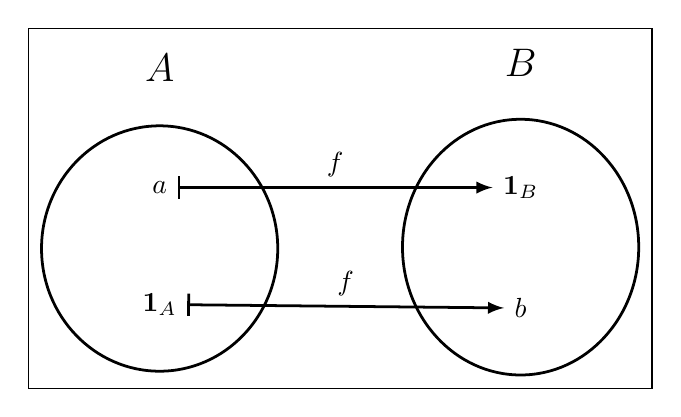
\begin{tikzpicture}[line width=1pt,>=latex, framed]
		\node (a) {$a$};
		\node[below=of a] (ida) {$\idarrow[A]$};
		
		\node[right=4 cm of a] (idb) {$\idarrow[B]$};
		\node[below=of idb] (b) {$b$};
		
		\node[shape=ellipse,draw=black,minimum size=3cm,fit={(ida) (a)}] {};
		\node[shape=ellipse,draw=black,minimum size=3cm,fit={(idb) (b)}] {};
		
		\node[above=1cm of a,font=\Large] {$A$};
		\node[above=1cm of idb,font=\Large] {$B$};
		
		\draw[|->] (a) -- (idb) node[midway,above] {$f$};
		\draw[|->] (ida) -- (b) node[midway,above] {$f$};
	\end{tikzpicture}
	\caption{The monoids $A$ and $B$, with elements and the isomorphism inbetween.\label{fig:1}}
\end{figure}

This shows that $b$ must be a left identity to $\idarrow[B]$. The same argument shows it is a right identity too. Next take an arbitrary $\beta \in B$, and you'll find that
$$ \beta = \idarrow[B] \times \beta = b \times \idarrow[B] \times \beta = b \times \beta$$
so clearly $b$ is a left identity in $B$ for all its members. An identical argument shows that it is a right identity in $B$. We can conclude that $b = \idarrow[B]$. 

Finally we conclude that $\idarrow[B] = f(\idarrow[A])$, and that finishes the challenge.





\end{ch}










%													CH 2
\begin{ch}\textit{Consider a monoid homomorphism from lists of integers with concatenation to integers with multiplication. What is the image of the empty list []? Assume that all singleton lists are mapped to the integers they contain, that is [3] is mapped to 3, etc. What’s the image of [1, 2, 3, 4]? How many different lists map to the integer 12? Is there any other homomorphism between the two monoids?}

Let $\cat C$ be the monoid of lists over $\nat$. Let $\cat D$ be the monoid of $\nat$ with multiplication, denoted $\times$. Let $g: \cat C \to \cat D$ be the monoid homomorhism described above.

We start with the first question: what is the image of the empty list? It is easy to deduce since it acts as identity with composistion. Let $l$ is some arbitrary list. Then
$$ g(l) = g( l ++ []) = g(l) * g([])$$
so clearly $g([]) = 1$.

Next, we want to find  $g([1,2,3,4]) $. This is an easy computation:
$$g([1,2,3,4]) = g([1])\times g([2])\times g([3])\times g([4]) = 1\times 2\times 3\times 4 = 24$$

Now we turn to the size of the preimage of $12$ under $g$. This must be the same as the number of (finite) lists over $\nat$ whose product is 12. It is quite stupid, since you can insert arbitrarily many $1$'s, so there are $\aleph_0$ such lists. Ignoring those, we only have $2\times 6$, $4\times 3$ and $2\times 2\times 3$ and unique permutations of that. We arrive at $7$ different lists.

The final question is both complicated and also easy. I'll chicken out on the complexity and argue like this: In the text, Bartosz states that list monoid is the free monoid. Next, when explaining the free monoid as a universal construction, he claims that the free monoid has a unique morphism to any other monoid $m$ with the same generator set. Since both monoids above have the generator $\nat$, the arrow between the monoids (as objects in $\cat{Mon}$), must be uinique.
\end{ch}











%													CH 3
\begin{ch}\textit{What is the free monoid generated by a one-element set? Can you see what it’s isomorphic to?}

First, remember that any universal construction does not make \emph{a} object, but rather \emph{a class} of objects that are uniquely isomorphic. Constructing a free monoid by universal construction, does therefore not get you \emph{the} free monoid, but rather $\emph{the free monoids}$. I the text, Bartosz states that the free monoid is the finite lists over the generator set plus the empty list. 

All one-element-sets are uniquely isomorphic, so we may choose any such set; lets pick ${()}$ as our one element set. Then the free monoid over ${()}$ is finite lists with all elements being $()$. Further, I claim that this is isomorphic to the nonnegative numbers $\nat ^0$ with addition. The one-to-one-mapping is between a list of $n$ elements and the number $n$. It is obviously a bijection, but to prove it formally, we must make sure it is a surjevtive and injective function. I won't bother do that...

As a last point, it might be fun to phrase it all in Haskell terms. Some googling says that this is actually not fun, but rather complicated. See for example : http://comonad.com/reader/2015/free-monoids-in-haskell/ 

But we might cheat a bit, go with Bartosz claim, and use list as the monoid. Then we could write:
\verbatiminput{freemonoid.hs}




\end{ch}

\end{document}